\documentclass[aspectratio=1610, xcolor=dvipsnames,handout]{beamer} %aspectratio=169, 
\usetheme{Pittsburgh}
\usepackage{tikz}
\usepackage{booktabs}
\usepackage[version=4]{mhchem}
\usepackage{animate}
\usepackage{biblatex}
\usepackage[absolute,overlay]{textpos}
\usepackage{fancyvrb}
\usepackage{xcolor}
\usepackage{multicol}
\usepackage{setspace}
\usepackage{siunitx}
\DeclareSIUnit\year{a}
\usepackage{qrcode}
\usepackage{eurosym}
\usepackage{xfrac}
\usepackage[export]{adjustbox}

% Thin fonts
\usepackage{cmbright}
\usepackage[T1]{fontenc}

\usetikzlibrary{arrows.meta}
\usetikzlibrary{shapes.geometric, arrows}
\urlstyle{same}

%gets rid of bottom navigation bars
\setbeamertemplate{footline}[frame number]{}
%gets rid of bottom navigation symbols
\setbeamertemplate{navigation symbols}{}

% colors
\definecolor{bokugreen}{rgb}{0.302, 0.675, 0.149}
\setbeamercolor{title}{fg=bokugreen, bg=white}
\setbeamercolor{frametitle}{fg=bokugreen}
\setbeamercolor{itemize item}{fg=bokugreen}
\setbeamercolor{enumerate item}{fg=bokugreen}
\setbeamercolor{local structure}{fg=bokugreen}


\newcommand{\backupbegin}{
   \newcounter{framenumberappendix}
   \setcounter{framenumberappendix}{\value{framenumber}}
}
\newcommand{\backupend}{
   \addtocounter{framenumberappendix}{-\value{framenumber}}
   \addtocounter{framenumber}{\value{framenumberappendix}} 
}

% title page
\setbeamertemplate{title page}[default][colsep=-4bp,rounded=true]
\title[The cost of undisturbed landscapes]{The cost of undisturbed landscapes}
\subtitle{Assessing systemic effects of renewables expansion in Austria}
\author{Sebastian Wehrle, Johannes Schmidt}
\institute{University of Natural Resources and Life Sciences, Vienna}
\date{February 25, 2020\\ \medskip NOeG Annual Meeting 2020}

%\setbeamertemplate{section page}{
%	\begin{center}
%	{\usebeamerfont[fg]{section title} \insertsection}
%	\end{center}
%}
\AtBeginSection[]{
  \begin{frame}
  \vfill
%  \centering
%  \begin{beamercolorbox}[sep=8pt,center,shadow=false,rounded=true]{title}
\tableofcontents[currentsection]
%\begin{textblock*}{10cm}(7cm, 2.0cm) % {block width} (coords)
%\adjincludegraphics[height=6cm,trim={0 0 {.3\width} 0},clip]{./figures/pv}
%\end{textblock*}
 %   \usebeamerfont{title} \usebeamercolor{title} \insertsection\par%
%  \end{beamercolorbox}
  \vfill
  \end{frame}
}

\begin{document}
    %%%%Title Page
    {
        \usebackgroundtemplate{
	        \begin{picture}(320,325)
    	        \hspace{9.0cm}
	              
\includegraphics[width=0.7\linewidth]{./logos/refuel_logo_with_text}
            \end{picture}
        }

        \begin{frame}[noframenumbering,plain]
          \maketitle
          \vspace{1.15cm}
          
\includegraphics[height=0.7cm]{./logos/creative-commons-by}
          \hspace{4.0cm}
\includegraphics[height=1.7cm]{./logos/boku-logo}\\
         \end{frame}
    }

\section{Background}
\begin{frame}
\frametitle{Austrian energy policy objectives}
\framesubtitle{according to government programme 2020-2024}
\begin{itemize}
\item 100\%\footnote[frame]{excluding system services and industry own consumption. At current levels this equals 10\% of consumption, i.e. actual target is around 90\%.} of electricity demand from domestic renewable sources on annual balance by 2030 \pause
\begin{itemize}
\item[$\rightarrow$] necessarily turns Austria into a net exporter of electricity \pause
\end{itemize}
\item additional annual electricity generation of \SI{27}{\tera\watt\hour} is expected to suffice \pause
\item technology-specific additions:
\end{itemize}

\begin{table}
\centering
\begin{tabular}{| l | r | r | r | r | r |}
\hline
 & 2018 & 2018\footnote[frame]{meteorological conditions as in 2016} & Policy & 2030 & 2030 \\ 
 & [GW] & [TWh] & [TWh] & [TWh] & [GW] \\ \hline \hline
Solar PV & 1.44 & 1.23 & +11 & 12.23 &  14.27 \\ \hline
Wind (onshore) & 3.05 & 6.14 & +10 & 16.14 & 8 \\ \hline
Hydro (run-of-river) & 5.72 & 28.34 & +5 & 33.34 & 6.73 \\ \hline
Biomass & $\sim 1$ & 4.78 & +1 & 5.78 & $>2$ \\ \hline
\end{tabular}
\end{table}
\end{frame}


\begin{frame}
\frametitle{Why wind is not solar}
\framesubtitle{A side note on imperfect substitutes}
%\begin{textblock*}{4cm}(0.75cm, 2.75cm)
%Aggregate profile for Austria
\begin{textblock*}{4cm}(0.75cm, 2.75cm)
\begin{itemize}
\item secure system operation requires $S=D$ at any point in time 
\item electricity not easily storable 
\item >>transforming<< electricity feed-in to end-use electricity is costly
\end{itemize}
\end{textblock*}

\only<2>{
\begin{textblock*}{10cm}(5.5cm, 2.25cm) % {block width} (coords)
\centering
Aggregate generation profile in Austria
\includegraphics[width=\textwidth, keepaspectratio]{./figures/wind_not_pv}
\end{textblock*}
}
\end{frame}



\begin{frame}
\frametitle{Stylized Facts}
\begin{itemize}
\item Apart from wind and solar, potentials for renewable electricity generation in Austria largely exhausted
\item Under announced policies, solar PV is only large-scale substitute to wind power \pause
\item Increasing social conflict around the large-scale expansion of onshore wind power
\item Traditional power system models do not account for local negative externalities of renewable energy generators, such as:
	\begin{itemize}
	\item visual impact on landscape
	\item harm to wildlife
	\item noise, flickering, glaring
	\end{itemize}
\end{itemize}
\end{frame}


\section{Motivation \& Method}
\begin{frame}
\frametitle{The problem from a social planner's perspective}
How to account for local negative externalities in renewables expansion planning?

\bigskip
\textcolor{bokugreen}{The cost of undisturbed landscapes}
\begin{itemize}
\item assess energy system effects and costs of substituting wind power with solar PV
\end{itemize}

\bigskip
\textcolor{bokugreen}{The value of undisturbed landscapes}
\begin{itemize}
\item estimates of the negative external effect of wind turbines reported in literature
\end{itemize}
\end{frame}


\begin{frame}
\frametitle{The cost of undisturbed landscapes}
\framesubtitle{Approach}
\begin{itemize}
\item Resemble Austrian power system in 2030
\item include most important electricity trading partner Germany \pause
\item set policy target of meeting $90\%$ of demand in 2030 from domestic renewable sources
\item incorporate announced electricity system targets for Germany in 2030
	\begin{itemize}
	\item nuclear phase-out
	\item partial coal exit
	\item expansion of renewable capacities in line with EEG 2017
	\end{itemize} \pause
\item simulate prospective electricity system with \emph{medea}
\end{itemize}
\end{frame}


\begin{frame}
\frametitle{Power system model \emph{medea}}
%\framesubtitle{Marketing slide}
\begin{footnotesize}
\begin{columns}[t]
\begin{column}{0.325\textwidth}
\textbf{Objective}
\begin{itemize}
\item minimize total system cost
	\begin{itemize}
	\begin{footnotesize}
	\item fuel and \ce{CO2} cost
	\item O\&M cost
	\item capital cost
	\end{footnotesize}
	\end{itemize}
\end{itemize}
\end{column}

\begin{column}{0.32\textwidth}  %%<--- here
\textbf{Decision variables}
\begin{itemize}
	\item hourly dispatch
	\item inter-zonal electricity trade
	\item investment in power plants, storages, and transmission
\end{itemize}
\end{column}

\begin{column}{0.32\textwidth}  %%<--- here
\textbf{Constraints}
\begin{itemize}
\item market clearing
\item capacity constraints
\item co-generation \& fuel use
%\item storage volume
\item system service requirement
\item inter-zonal electricity trade
\end{itemize}
\end{column}
\end{columns}
\end{footnotesize}
\bigskip
\begin{footnotesize}
\begin{columns}[t]
\begin{column}{0.325\textwidth}
\textbf{Economic assumptions}
\begin{itemize}
\item perfect competition
\item perfect foresight
\item price-inelastic demand
\end{itemize}
\end{column}

\begin{column}{0.325\textwidth}
\textbf{Resolution}
\begin{itemize}
\item hours (one year)
\item bidding zones
\item 41 technologies
\end{itemize}
\end{column}

\begin{column}{0.325\textwidth}
\textbf{Implementation}
\begin{itemize}
\item linear program
\item python \& GAMS
\end{itemize}
\end{column}
\end{columns}
\end{footnotesize}
\bigskip

\medskip
\begin{center}
\emph{medea} is available on \href{https://github.com/inwe-boku/medea}{github.com/inwe-boku/medea} under an open MIT license
\end{center}
\end{frame}
\note{
medea is a partial-equilibrium model of the coupled electricity and district heating sectors.
Operation of and investment in conventional and renewable power plants, storages and transmission lines are determined simultaneously for one year.
Results include hourly dispatch, investment, inter-zonal trade, electricity and heat prices, profits, and emissions of air pollutants.
The model accounts for various technical characteristics of power systems, such as co-generation of heat and power, balancing requirements, 
}


\begin{frame}
\frametitle{The cost of undisturbed landscapes}
\framesubtitle{Estimating the opportunity cost of wind power}
\begin{itemize}
\item[1)] derive unrestricted optimal deployment of wind and solar power
\item[2)] restrict deployment of wind power by a small margin \\($\rightarrow$ solar PV substitutes for wind)
\item[3)] repeat till no wind power can be deployed
\end{itemize}

\bigskip
We approximate the cost of undisturbed landscapes (i.e. the forgone value of wind power $w$) by the change in net cost of the electricity system including air pollution cost $c_{net}$ in response to a change in deployed wind power $w$, i.e.
\begin{align*}
oc_w = \frac{\Delta c_{net}}{\Delta w}
\end{align*}

\end{frame}


\section{Results}
\begin{frame}
\frametitle{The cost of undisturbed landscapes}

\begin{textblock*}{10cm}(0.75cm, 1.5cm) % {block width} (coords)
\includegraphics[width=\textwidth, keepaspectratio]{./figures/undisturbed_base}
\end{textblock*}

\begin{textblock*}{4.5cm}(10.9cm, 1.5cm)
\begin{small}
\begin{table}
\begin{tabular}{p{1.8cm} | r l}
Capital cost of solar PV & $630$ & \SI{}{\text{\euro}\per\kilo\watt\text{p}}
\end{tabular}
\end{table}
\smallskip
\quad $\rightarrow$ about $\sfrac{2}{3}$ rooftop PV, \\
\quad $\sfrac{1}{3}$ open space PV

\vspace{4.25cm}
\quad wind power and solar PV \\ \quad are substitutes
\end{small}
\end{textblock*}

\begin{textblock*}{9.5cm}(1.5cm, 8.2cm)
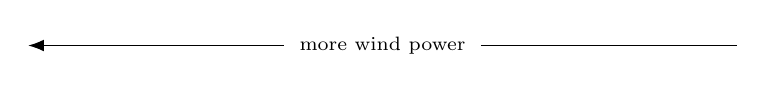
\begin{tikzpicture}%[thick]
\draw (5.75,0) -- (9,0);
\draw[{Latex[length=2mm]}-] (0,0) -- (3.25,0);
\draw (4.5,0.0) node[] {\scriptsize more wind power};
\end{tikzpicture}

\begin{tikzpicture}%[thick]
\draw[-{Latex[length=2mm]}] (5.5,0) -- (9,0);
\draw (0,0) -- (3.5,0);
\draw (4.5,0.0) node[] {\scriptsize more solar PV};
\end{tikzpicture}
\end{textblock*}

\end{frame}


\begin{frame}
\frametitle{The cost of undisturbed landscapes}
\framesubtitle{Cost with restricted wind power}
\begin{textblock*}{10cm}(0.75cm, 2.0cm) % {block width} (coords)
\includegraphics[width=\textwidth, keepaspectratio]{./figures/cost}
\end{textblock*}

\begin{textblock*}{4cm}(11cm, 2.25cm)
\begin{small}
\begin{table}
\begin{tabular}{p{1.8cm} | p{0.3cm} l}
Capital cost of solar PV & $630$ & \SI{}{\text{\euro}\per\kilo\watt\text{p}} \\
\ce{CO2} price & $90$ & \SI{}{\text{\euro}\per\mega\watt\hour}
\end{tabular}
\end{table}
\end{small}
\end{textblock*}

\end{frame}


\begin{frame}
\frametitle{The cost of undisturbed landscapes}
\framesubtitle{System operation with restricted wind power}
\begin{textblock*}{10cm}(0.75cm, 2.0cm) % {block width} (coords)
\includegraphics[width=\textwidth, keepaspectratio]{./figures/sysops}
\end{textblock*}

\begin{textblock*}{4cm}(11cm, 2.25cm)
\begin{small}
\begin{table}
\begin{tabular}{p{1.8cm} | p{0.3cm} l}
Capital cost of solar PV & $630$ & \SI{}{\text{\euro}\per\kilo\watt\text{p}} \\
\ce{CO2} price & $90$ & \SI{}{\text{\euro}\per\mega\watt\hour}
\end{tabular}
\end{table}
\end{small}
\end{textblock*}

\end{frame}


\section{Sensitivity}
\begin{frame}
\frametitle{The cost of undisturbed landscapes}
\framesubtitle{Sensitivity to capital cost of solar PV}
\begin{textblock*}{10cm}(0.75cm, 2.0cm) % {block width} (coords)
\includegraphics[width=\textwidth, keepaspectratio]{./figures/sens_nrg}
\end{textblock*}

\begin{textblock*}{4cm}(11cm, 2.25cm)
\begin{small}
Capital cost estimates for solar PV in 2030
\begin{table}
\begin{tabular}{p{1.8cm} | p{0.3cm} l}
Small-scale rooftop & $830$ & \SI{}{\text{\euro}\per\kilo\watt\text{p}} \\
Utility-scale open space & $280$ & \SI{}{\text{\euro}\per\kilo\watt\text{p}} \\
\end{tabular}
\end{table}
\end{small}
\end{textblock*}
\end{frame}


\begin{frame}
\frametitle{The cost of undisturbed landscapes}
\framesubtitle{Sensitivity to capital cost of solar PV}
\begin{textblock*}{10cm}(0.75cm, 2.0cm) % {block width} (coords)
\includegraphics[width=\textwidth, keepaspectratio]{./figures/undisturbed_low}
\end{textblock*}

\begin{textblock*}{4cm}(11cm, 2.25cm)
\begin{small}
\begin{table}
\begin{tabular}{p{1.8cm} | p{0.3cm} l}
Capital cost of solar PV & $280$ & \SI{}{\text{\euro}\per\kilo\watt\text{p}}
\end{tabular}
\end{table}
\end{small}
\end{textblock*}
\end{frame}


\section{Discussion \& Conclusion}
\begin{frame}
\frametitle{The cost of undisturbed landscapes}
\framesubtitle{Discussion of results}
\begin{itemize}
\item Renewable resource quality held constant as capacity is expanded
\item Sub-national electricity transmission and distribution grids neglected
\item Technical operation of generators not fully represented \\(e.g. no unit commit, simplified balancing)
\item Electricity market-splitting has increased market concentration
\item Announced policy necessarily turns Austria into a net exporter of electricity\\
$\rightarrow$ "loop-flows" potentially avoided \\
$\rightarrow$ artificial transmission restriction between DE and AT could be eliminated
%\item use Austrian landscape for "overinvesting" in wind and exporting to Germany?
\end{itemize}
\end{frame}


\begin{frame}
\frametitle{Conclusions}
\begin{itemize}
\item If we value \ce{CO2} emissions at 30 \SI{}{\text{\euro}\per\mega\watt\hour} or lower, onshore wind power can be substituted by open-space utility-scale solar PV at little loss
% and approve of open-space utility-scale solar PV, onshore wind power is sub-optimal

\item \ce{CO2} valuation above 30 \SI{}{\text{\euro}\per\mega\watt\hour} or a preference for rooftop PV allows for gains to be made from wind power deployment

\item Gains from wind power could be used to compensate the ones affected by local negative externalities of wind turbines

\item Complementing our analysis with spatially resolved estimates of wind turbine impacts, one could derive a spatially explicit plan for the socially optimal expansion of wind power in Austria
\end{itemize}
\end{frame}


 %%%Last Frame
 {
    \usebackgroundtemplate{
        \begin{picture}(320,290)
        \hspace{9.5cm}
          
\includegraphics[width=0.6\linewidth]{./logos/refuel_logo_with_text}
%        \begin{picture}(200,305)
%        \hspace{7.7cm}
%          
\includegraphics[width=0.6\linewidth]{refuel_logo_with_text}
        \end{picture}
    }
    \begin{frame}
        \frametitle{Thank you!}
        \vspace{0.5cm}
        \url{https://refuel.world}\\
        \url{https://github.com/inwe-boku/medea}\\
        \url{sebastian.wehrle@boku.ac.at}

		\vspace{0.6cm}
        \qrcode[height=2cm]{http://github.com/inwe-boku/medea}\\

        \vspace{1.65cm}
        
\includegraphics[height=0.7cm]{./logos/creative-commons-by}
        
        \smallskip
        \tiny{We gratefully acknowledge support from the European Research Council \\(“reFUEL” ERC-2017-STG 758149).}

    \end{frame}
}   
%\appendix
%\backupbegin
%
%
%\begin{frame}
%\frametitle{The cost of undisturbed landscapes}
%\framesubtitle{Unconstrained deployment of wind and solar power}
%
%\begin{textblock*}{10cm}(0.75cm, 1.8cm) % {block width} (coords)
%\begin{table}
%\begin{tabular}{l r l}
%\emph{Results for Austria} \\ \hline \hline
%Added Solar PV & 0.0 & \SI{}{\tera\watt\hour} \\ \hline
%Added Wind & 31.0 & \SI{}{\tera\watt\hour} \\ \hline \hline
%System Cost\footnote[frame]{excluding cost for domestic transmission and distribution grids} & $3095.2$ & \SI{}{\mega\text{\euro}} \\ \hline
%Trade balance & $746.8$ & \SI{}{\mega\text{\euro}} \\ \hline
%Cost of air pollution & $184.4$ & \SI{}{\mega\text{\euro}} \\ \hline
%\ce{CO2} emissions & $5227.3$ & \SI{}{\kilo\tonne} \\ \hline
%Electricity generation & $92.8$ & \SI{}{\tera\watt\hour} \\ \hline
%Curtailment & $2.4$ & \SI{}{\tera\watt\hour} \\ \hline
%Net exports & $5.9$ & \SI{}{\tera\watt\hour} \\ \hline
%Wholesale electricity price & $56.05$ & \SI{}{\text{\euro}\per\mega\watt\hour} \\ \hline
%\end{tabular}
%%\caption{Results for Austria}
%\end{table}
%\end{textblock*}
%
%\begin{textblock*}{4cm}(11cm, 2.05cm)
%\begin{small}
%\begin{table}
%\begin{tabular}{p{1.8cm} | p{0.3cm} l}
%Capital cost of solar PV & $630$ & \SI{}{\text{\euro}\per\kilo\watt\text{p}} \\
%\ce{CO2} price & $90$ & \SI{}{\text{\euro}\per\mega\watt\hour}
%\end{tabular}
%\end{table}
%\end{small}
%\end{textblock*}
%
%\end{frame}
%
%
%\begin{frame}
%\frametitle{The value of undisturbed landscapes}
%\framesubtitle{Local Negative Externalities of Wind Turbines}
%%\begin{table}[h!]
%%\caption{Estimates of Wind Turbine Impact on Property Prices}
%\begin{table}
%\centering
%\begin{scriptsize}
%	\begin{tabular}{p{3.2cm} l l l p{1.1cm} p{2.4cm}}
%	\hline
%	Authors & Country & Sample & Framework\footnote[frame]{DID $\ldots$ difference-in-differences, SAR $\ldots$ spatial autoregressive, SFE $\ldots$ spatial fixed effects} & Impact Proxy\footnote[frame]{d $\ldots$ distance, v $\ldots$ visibility} & Estimated Impact \\
%	\hline \hline
%%	\cite{Sims2008} & Cornwall, UK & 2000 - 2007 & hedonic & visibility dummies & insignificant \\ \hline
%	Heintzelmann and Tuttle, 2012 & USA, NY & 2000 - 2009 & hedonic, SFE & d & $-3.6\%$ to $-9.6\%$, insignificant \\ \hline
%	Jensen et al., 2014 & DNK & 2000 - 2011 & hedonic, SAR & d, v & $-4.35\%$ \\ \hline
%	Lang et al., 2014 & USA, RI & 2000 - 2013 & DID & d, v & insignificant  \\ \hline
%	Gibbons, 2015 & GBR, EAW & 2000 - 2011 & DID & d, v & $-6\%$ \\ \hline
%	Hoen et al., 2015 & USA & 1996 - 2011 & DID & d & insignificant \\ \hline
%	Dröes and Koster, 2016 & NED & 1985 - 2011 & DID & d & $-1.4\%$\\ \hline
%	Sunak and Madlener, 2016 & GER, NRW & 1992 - 2010 & DID & v & $-9\%$ to $-14\%$ \\ \hline
%	Jensen et al., 2018 & DNK & - & hedonic, SAR & d, \# of turbines & $-0.2\%$ to $-1.1\%$ \\ \hline
%	Kussel et al., 2019 & GER & 2007 - 2015 & DID & d & $-6.0\%$ \\ \hline \hline
%	\end{tabular}
%%\label{tab:negex}
%\end{scriptsize}
%\end{table}
%\end{frame}
%
%
%\begin{frame}
%\frametitle{Compensating for local negative externalities}
%\framesubtitle{An example}
%\begin{textblock*}{7cm}(0.75cm, 2.0cm) % {block width} (coords)
%OC of wind turbines in Austria
%\vspace{-0.41cm}
%\begin{table}
%%\centering
%\begin{footnotesize}
%	\begin{tabular}{c | c | c | c}
%	$oc_w$ & $\delta$ & NPV $oc_w$ & NPV $oc_w$ \\
%	$[\text{\euro}\, \text{MW}^{-1} \text{a}^{-1}]$ & & $[\text{\euro}\, \text{MW}^{-1}]$ & $[\text{\euro} \, \text{turbine}^{-1}]$ \\ \hline \hline
%	$40\,000$ & $0.05$ & $563\,758$ & $1\,973\,152$ \\ \hline
%	$40\,000$ & $0.03$ & $696\,526$ & $2\,437\,841$ \\ \hline
%	$10\,000$ & $0.05$ & $140\,939$ & $493\,288$ \\ \hline
%	$10\,000$ & $0.03$ & $171\,131$ & $609\,460$ \\ \hline
%	\end{tabular}
%\end{footnotesize}
%\end{table}
%\end{textblock*}
%
%\begin{textblock*}{7cm}(8.25cm, 2.0cm) % {block width} (coords)
%Property value loss in Germany
%%\vspace{-0.5cm}
%\begin{table}
%%\centering
%\begin{footnotesize}
%	\begin{tabular}{c | c | c | c}
%	  & value & impact & loss \\
%	  & \euro & \% & \euro \\ \hline \hline
%	mean & $273\,786$ & $0.06$ & $16\,427$ \\ \hline
%	mean & $273\,786$ & $0.10$ & $27\,379$ \\ \hline
%	mean + 1 s.d. & $476\,923$ & $0.06$ & $28\,615$ \\ \hline
%	mean + 1 s.d. & $476\,923$ & $0.10$ & $47\,692$ \\ \hline
%	\end{tabular}
%\end{footnotesize}
%\end{table}
%\end{textblock*}
%
%\begin{textblock*}{14.5cm}(0.75cm, 6.0cm) % {block width} (coords)
%\centering
%Compensation potential
%\vspace{-0.1cm}
%\begin{table}
%\begin{footnotesize}
%	\begin{tabular}{c | c | c | c | c}
%	$oc_w$  & $\delta$ & value & impact & \# property owners \\ \hline \hline
%	$40\,000$ & $0.05$ & $273\,786$ & $0.06$ & $120$ \\ \hline
%	$40\,000$ & $0.05$ & $273\,786$ & $0.10$ & $72$ \\ \hline
%	$40\,000$ & $0.03$ & $476\,923$ & $0.06$ & $69$ \\ \hline
%	$40\,000$ & $0.03$ & $476\,923$ & $0.10$ & $41$ \\ \hline
%%	$10\,000$ & $0.05$ & $476\,923$ & $0.06$ & $1$ \\ \hline
%	$10\,000$ & $0.03$ & $476\,923$ & $0.10$ & $18$ \\ \hline
%	\end{tabular}
%\end{footnotesize}
%\end{table}
%\end{textblock*}
%
%\end{frame}
%\backupend
\end{document}